\chapter{Introduction}\label{ch:1}

  Classification, in the context of machine learning, deals with the problem of 
  predicting the class of a set of examples given their features. Traditionally, classification 
  methods aim at minimizing the misclassification of examples, in which an example is 
  misclassified if the predicted class is different from the true class. Such a traditional 
  framework assumes that all misclassification errors carry the same cost. This is not the case in 
  many real-world applications. Methods that use different misclassification costs are known as 
  cost-sensitive classifiers. Typical cost-sensitive approaches assume a constant cost for each 
  type of error, in the sense that, the cost depends on the class and is the same among examples 
  \citep{Elkan2001,Kim2012}. 
  
  This class-dependent approach is not realistic in many real-world applications. For 
  example in credit card fraud detection, failing to detect a fraudulent transaction may have an 
  economical impact from a few to thousands of Euros, depending on the particular transaction and 
  card holder \citep{Ngai2011a}. In churn modeling, a model is used for predicting which
  customers are more likely to abandon a service provider. In this context, failing to identify a 
  profitable or unprofitable churner has a significant different economic 
  result~\citep{Verbraken2013}. Similarly, in direct marketing, wrongly predicting that a customer 
  will not accept an offer when in fact he will, may have different financial impact, as not all 
  customers generate the same profit \citep{Zadrozny2003}. Lastly, in credit scoring, accepting 
  loans from bad customers does not have the same economical loss, since customers have different 
  credit lines, therefore, different profit \citep{Verbraken2014}.
  
  Methods that use different misclassification costs are known as cost-sensitive classifiers. In 
  particular we are interested in methods that are example-dependent cost-sensitive, in the sense 
  that the costs vary among examples and not only among classes \citep{Elkan2001}. However, the 
  literature on example-dependent cost-sensitive methods is limited, mostly because there is a 
  lack of publicly available datasets that fit the problem \citep{MacAodha2013}.
  Example-dependent cost-sensitive classification methods can be grouped according to the step 
  where the costs are introduced into the system. Either the costs are introduced prior to the 
  training of the algorithm, after the training or during training \citep{Wang2013}. In 
  \figurename{ \ref{fig:1:1}}, the different algorithms are grouped according to the stage in a 
  classification system where they are used.
  
  The first set of methods that were proposed to deal with cost-sensitivity consist in 
  re-weighting the training examples based on their costs, either by cost-proportionate 
  rejection-sampling \citep{Zadrozny2003}, or cost-proportionate over-sampling \citep{Elkan2001}.
  The rejection-sampling approach consists in selecting a random subset by randomly 
  selecting examples from a training set, and accepting each example with probability equal to 
  the normalized misclassification cost of the example. On the other hand, the over-sampling 
  method consists in creating a new set, by making $n$ copies of each example, where $n$ is related 
  to the normalized misclassification cost of the example.
  In \citep{CorreaBahnsen2013,CorreaBahnsen2014}, we proposed a direct cost approach to make the 
  classification decision based on the expected costs. This method is called Bayes minimum risk, and 
  has been successfully applied to detect credit card fraud. The method   
  consists in quantifying tradeoffs between various decisions using probabilities and the costs   
  that accompany such decisions. 
  
  Moreover, in \citep{CorreaBahnsen2014b}, we proposed a new cost-sensitive logistic regression. 
  The   method consists in introducing example-dependent costs into a logistic regression, by 
  changing   the objective function of the model to one that is  cost-sensitive. 
  Then, in \citep{CorreaBahnsen2015}, we proposed a new example-dependent cost-sensitive decision 
  tree. The method is based on a new splitting criteria which is cost-sensitive, used during the 
  tree construction. Then, after the tree is fully grown, it is pruned by using a cost-based 
  pruning criteria. Lastly, in \citep{CorreaBahnsen2015b}, we proposed a ensemble of cost-sensitive 
  decision tree framework. This is an extension of the previously proposed methods, in which the 
  advantages of ensemble learning are used in order to have a more robust model.

  \begin{figure}
  \centering
    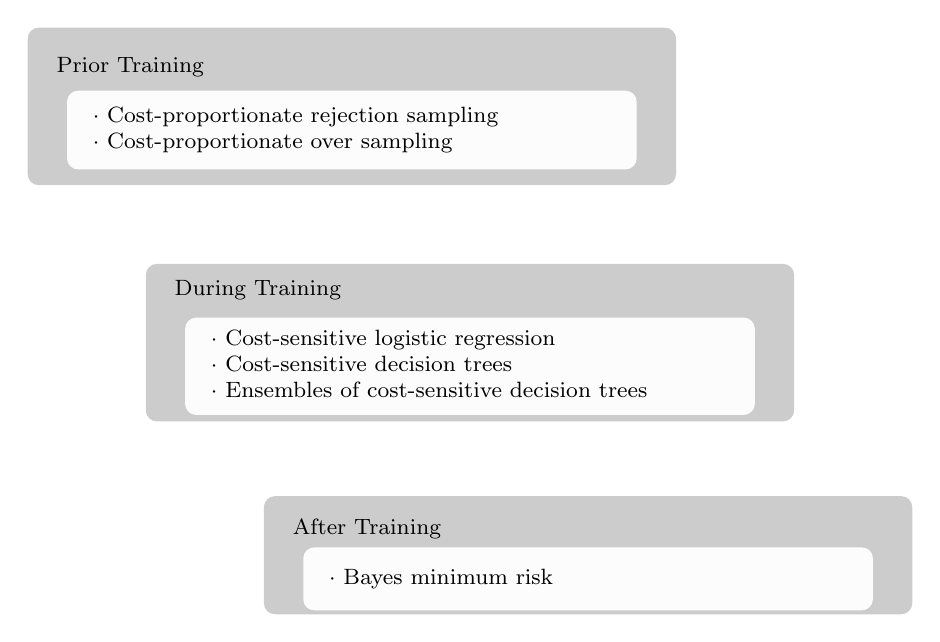
\begin{tikzpicture}[node distance=2.5cm]
  \tikzstyle{every node}=[font=\footnotesize]
  
  % Main boxes
  \node (data1) [rectangle, rounded corners, minimum width=2cm, minimum height=2cm,text 
                centered, fill=black!20, text width=8cm] 
                {\tabular{p{7.5cm}} Prior Training\\ \\ \\ \\ \endtabular};
  \node (data2) [rectangle, rounded corners, minimum width=2cm, minimum height=2cm,text 
                centered, fill=black!20, right of=data1, yshift=-3cm, xshift=-1cm, text 
                width=8cm] {\tabular{p{7.5cm}} During Training\\ \\ \\ \\ \\ \endtabular};
  \node (data3) [rectangle, rounded corners, minimum width=2cm, minimum height=1.5cm,text 
                centered, fill=black!20, right of=data2, yshift=-2.7cm, xshift=-1cm, text 
                width=8cm] {\tabular{p{7.5cm}} After Training\\ \\ \\ \endtabular};

  \node (data11) [rectangle, rounded corners, minimum width=2cm, minimum height=1cm, 
                fill=black!1, below of=data1, yshift=2.2cm, text width=7cm]
                {\tabular{p{7cm}} $\cdot$ Cost-proportionate   rejection sampling \\ 
                $\cdot$ Cost-proportionate over sampling \endtabular};

  \node (data21) [rectangle, rounded corners, minimum width=2cm, minimum height=1cm, 
                fill=black!1, below of=data2, yshift=2.2cm, text width=7cm]
                {\tabular{p{7cm}} $\cdot$ Cost-sensitive logistic regression \\
                $\cdot$ Cost-sensitive decision trees \\ 
                $\cdot$ Ensembles of cost-sensitive decision trees \endtabular};
  
  \node (data31) [rectangle, rounded corners, minimum width=2cm, minimum height=0.8cm, 
                fill=black!1, below of=data3, yshift=2.2cm, text width=7cm]
                {\tabular{l} $\cdot$ Bayes minimum risk  \endtabular};
	
	% Arrows
% 	\draw[thick,->,>=stealth] (data1) to (data2);
%   \draw[thick,->,>=stealth] (data2) to (data3);
  \end{tikzpicture}
 
%  \tikzstyle{startstop} = [rectangle, rounded corners, minimum width=2cm, minimum height=4cm,text 
% centered, draw=black, fill=black!20]
% \tikzstyle{startstop2} = [rectangle, rounded corners, minimum width=2cm, minimum height=1cm,text 
% centered, draw=black, fill=black!20]
% \tikzstyle{startstop3} = [rectangle, rounded corners, minimum width=2cm, minimum height=2.9cm,text 
% left, draw=black, fill=black!1]
% \tikzstyle{arrow} = [thick,->,>=stealth]
  \caption{Different example-dependent cost-sensitive algorithms grouped according to the 
    stage in a classification system where they are used.}
  \label{fig:1:1}
  \end{figure}
  
  We evaluate the different methods using five different databases from four real-world problems. In 
  particular, credit card fraud detection, churn modeling, credit scoring and direct marketing. 
  The results show that the proposed method outperforms state-of-the-art  example-dependent   
  cost-sensitive methods. Furthermore, our source code, as used for the experiments, is publicly 
  available as part of the \textit{CostSensitiveClassification}\footnote{
  \url{https://github.com/albahnsen/CostSensitiveClassification}} library.
  
  The results show that by taking into account the real financial costs of the different 
  real-world applications, our  proposed example-dependent cost-sensitive decision tree is a better 
  choice for these and many other applications. This is because, our algorithm is focusing on 
  solving the actual business problems,  and not proxies as standard classification models do. We 
  foresee that our approach should open the door to developing more business focused algorithms, 
  and  that ultimately, the use of the actual financial costs during training will become a common 
  practice. Moreover, by creating many different decision trees and combining them using a 
  cost-sensitive ensemble framework, the best results are found.

  Finally, our results show the importance of using the real example-dependent financial costs 
  associated with real-world applications, since there are significant differences in the 
  results when evaluating a model using a traditional cost-insensitive measure such as the 
  accuracy or F1Score,  than when using the savings, leading to the conclusion of the 
  importance of using the real practical financial costs of each context.

\newpage
\section{Outline and contributions}

\todo{add part 1}

\chaptername{ \ref{ch:background}} is focused in giving the general concepts of classification 
and cost-sensitive classification. In particular, define what is the different between 
cost-insensitive, class-dependent cost-sensitive and example-dependent cost-sensitive 
classification problems. Moreover, we give an introduction of the different evaluation measures 
that are used throughout this thesis.

\partname{~\textsc{\ref{part:1}}} is dedicated to explain the particularities of the four 
real-world classification problems that are the focus of this thesis, in particular, credit card 
fraud detection, credit scoring, churn modeling and direct marketing. In general, we show why each 
of the applications is example-dependent cost-sensitive, and we elaborate a framework for the 
analysis of each problem. The Part is organized in two Chapters. First, in 
\chaptername{~\ref{ch:3}}, we discussed the applications within financial risk management. Lastly, 
in  \chaptername{~\ref{ch:4}}, the marketing analytics applications.

\partname{~\textsc{\ref{part:2}}} is focused in introducing our proposed example-dependent 
cost-sensitive methods. First, in \chaptername{~\ref{ch:5}}, we present our Bayes minimum risk 
method. Then, in \chaptername{~\ref{ch:6}}, we introduce our method cost-sensitive logistic 
regression. Afterwards, in \chaptername{~\ref{ch:7}}, we show and discuss our previously proposed 
cost-sensitive decision trees algorithm. Furthermore, in \chaptername{~\ref{ch:8}}, we explain our 
proposed framework for ensembles of cost-sensitive decision trees. Lastly, in 
\chaptername{~\ref{ch:9}}, we present the library \mbox{\textit{CostCla}} that we develop as part of 
the thesis. This library is an open-source implementation of all the algorithms covered in this 
manuscript.

\chaptername{ \ref{ch:10}} concludes the thesis, and elaborates on possible lines for future 
research.

\section{Publications}

This dissertation summarizes several contributions to the field of example-dependent 
cost-sensitive machine learning. Publications from this work include:
\bigskip

\begin{itemize}
\item \citep{CorreaBahnsen2013} \textit{Cost Sensitive Credit Card Fraud Detection Using Bayes 
Minimum Risk}, Alejandro Correa Bahnsen,  Aleksandar Stojanovic, Djamila Aouada and Bj\"orn 
Ottersten. In Proceedings of IEEE International Conference on Machine Learning and Applications, 
2013.

\item \citep{CorreaBahnsen2014} \textit{Improving Credit Card Fraud Detection with Calibrated 
Probabilities}, Alejandro Correa Bahnsen, Djamila Aouada and Bj\"orn Ottersten.
In Proceedings of SIAM International Conference on Data Mining, 2014.

\item \citep{CorreaBahnsen2014b} \textit{Example-Dependent Cost-Sensitive Logistic Regression for 
Credit Scoring}, Alejandro Correa Bahnsen, Djamila Aouada and Bj\"orn Ottersten.
In Proceedings of IEEE International Conference on Machine Learning and Applications, 2014.

\item \citep{CorreaBahnsen2015} \textit{Example-Dependent Cost-Sensitive Decision Trees},
Alejandro Correa Bahnsen, Djamila Aouada and Bj\"orn Ottersten.
In Expert Systems with Applications, in press, 2015.

\item \citep{CorreaBahnsen2015a} \textit{A novel cost-sensitive framework for customer churn 
predictive modeling}, Alejandro Correa Bahnsen, Djamila Aouada and Bj\"orn Ottersten.
In Decision Analytics, 2015.

\item \citep{CorreaBahnsen2015b} \textit{Ensembles of Example-Dependent Cost-Sensitive Decision 
Trees}, Alejandro Correa Bahnsen, Djamila Aouada and Bj\"orn Ottersten.
In IEEE Transactions on Knowledge and Data Engineering, 2015.

\item \citep{CorreaBahnsen2015c} \textit{Feature Engineering in Credit Card Fraud Detection},
Alejandro Correa Bahnsen, Djamila Aouada and Bj\"orn Ottersten. In Expert Systems with 
Applications, 2015.

\end{itemize}
